\section{Stars \& Stellar Astrophysics}

\begin{sectionauthor}
   Dr. Candice Stauffer (Northwestern University PhD) 
\end{sectionauthor}
\vspace{20pt}

Stars are born, they change, grow and evolve over time, and perhaps most surprisingly to a lot of us -- stars die.
However, for some at least, death is not the end but rather a new chapter in the great book of stellar astrophysics. 
Let me take you back to the very start.


\subsection{Stellar Evolution}
 
\subsubsection{Birth}

Stars are born in a complex process that begins deep in the cosmos from vast, cold clouds of gas and dust called nebulae. Over time, something very interesting begins to happen in these nebulae. Due to the gravitational pull, the particles of these clouds begin to clump together, forming \textbf{giant molecular clouds}. As they gather, they create denser regions. As the density in those regions increases, the gravity becomes stronger, pulling even more gas and dust, making the clumps larger. Typical giant molecular clouds are roughly \(9.5 \times 10^{14}\) km across, a distance so vast that light, the fastest thing in the universe, would take a century to traverse it. In terms of mass, these clouds typically contain about \(10^4\) to \(10^6\) times the mass of our Sun\footnote{Mass is typically compared to the mass of the Sun: $1.0\,\mathrm{M_{\odot}}$ ($2.0\times 10^{30}\;\mathrm{kg}$) means 1 solar mass.}.


As the very core of these clumps grow even hotter and denser, the star formation process begins. The core of the giant molecular cloud begins to collapse and as this occurs, it breaks into smaller and smaller pieces. In each of these fragments, the collapsing gas releases gravitational potential energy as heat. As its temperature and pressure increase, a fragment condenses into a rotating ball of superhot gas known as a \textbf{protostar}. At this stage, the protostar is a hot, dense ball of gas and dust, glowing with heat but not yet shining with the steady light of a mature star. It's like a star in the making, going through its early developmental stages.

As the protostar matures, its core reaches a critical juncture of density and temperature — a pivotal moment in the birth of a star. During this transformative phase, the protostar continues to draw in mass from the surrounding nebula, growing larger and more massive. With this growth, the pressure and temperature within its core escalate steadily, setting the stage for a stellar spectacle.

This period is crucial in a star's life cycle. If the protostar acquires sufficient mass, the core's temperature will eventually soar to such extremes that it ignites a remarkable process: hydrogen atoms, under intense heat and pressure, start to merge, forming helium. This process, known as \textbf{nuclear fusion}, is akin to striking a match on a vast cosmic scale, sparking a brilliant and sustained glow. Nuclear fusion unleashes an immense surge of energy, which is the secret behind a star's radiance.

\begin{figure}[h!]
    \centering
    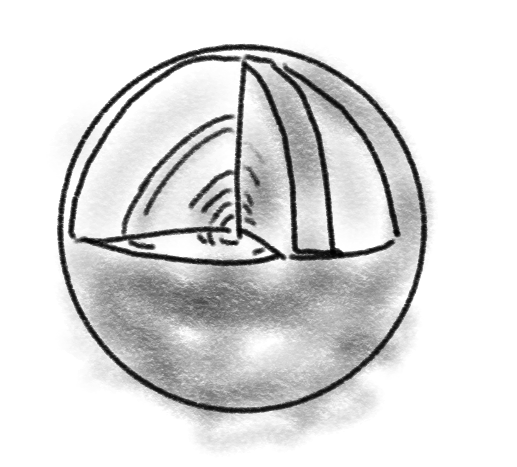
\includegraphics[width=0.4\linewidth]{img/star.png}
    \caption{Stars are structured in radial layers defined by a gradient in temperature and density. For post-main sequence stars, this also translates to a chemical gradient, with the heavier elements in the star's fusing core and the lightest elements in the star's outer layers.}
    \label{fig:star}
\end{figure}

Imagine lighting a colossal furnace that can blaze for millions, even billions of years. That's what happens when a star is born. This fusion process not only lights up the star but also marks the commencement of its extensive journey, a journey spent predominantly in converting hydrogen into helium, fueling its luminous presence in the universe.

This is just the beginning of a star's life. Depending on its size, a star can live for a few million years if it's really big, or for tens of billions of years if it's more like our Sun. Over its lifetime, a star will undergo various changes, eventually leading to its death, which is another remarkable story in itself.

\subsubsection{Life}
Stars are classified into different types based on their temperature, color, and size. A common mnemonic to remember these types is `OBAFGKM,' where each letter represents a class of stars — O, B, A, F, G, K, and M.\footnote{An easy way to remember the order of the 'OBAFGKM' mnemonic is with the phrase: 'Only Boring Astronomers Fight Green Killer Martians'.} These classes range from the hottest, most massive O-type stars to the cooler, smaller M-type stars, essentially forming a temperature scale for stars.

In the heart of every star, a remarkable process occurs: nuclear fusion. This is the key to a star's life, akin to the burning flame in a fireplace; it's what makes them shine and prevents gravity from collapsing them into a mere point. During their main sequence phase, stars spend most of their lifetime fusing hydrogen into helium in their cores. This phase is stable and can last from a few million years for massive O-type stars to tens of billions of years for smaller M-type stars.

As stars exhaust their hydrogen fuel, they evolve off the main sequence. Their composition subtly shifts, with the core, now rich in helium, moving on to fuse this new element. Meanwhile, hydrogen fusion continues in a shell surrounding the core. For instance, a star like our Sun (a G-type star) will eventually swell into a red giant, fusing helium into heavier elements. Larger O and B-type stars, due to their massive size and higher core pressure and temperature, can fuse elements all the way up to iron.

However, there is a limit. The fusion of iron in the most massive stars marks a turning point. Iron fusion consumes more energy than it releases, effectively halting the fusion process. This is a critical juncture in a star's life. Stars like our Sun, with about a solar mass, exhaust their nuclear fuel and shed their outer layers in a planetary nebula. The remaining dense core collapses into a white dwarf.

In contrast, stars more than ten times the mass of the Sun meet a dramatic end. They explode in \textbf{supernovae}, events so powerful they briefly outshine entire galaxies. The aftermath of such an explosion leaves behind either a neutron star — an incredibly dense object composed of neutrons — or, for the most massive stars, a black hole, an entity with gravity so strong that not even light can escape it.

This stellar lifecycle is a testament to the dynamic and ever-changing nature of the universe, reflecting the delicate balance of forces and intricate processes that govern the life and death of the stars illuminating our night sky.


\subsection{Stellar Graveyards}
\subsubsection{Death}

As stars reach the end of their lives, they undergo remarkable transformations, leading to various final stages depending on their initial mass. Two notable outcomes are white dwarfs and neutron stars, each a fascinating testament to the laws of physics operating under extreme conditions.

\subsubsection{White Dwarfs}

A white dwarf represents the final evolutionary stage of medium-sized stars, like our Sun. When such stars exhaust their nuclear fuel, they shed their outer layers, leaving behind a hot, dense core. This core becomes a white dwarf. Despite being small in size, white dwarfs are incredibly dense. A white dwarf's mass is comparable to that of the Sun, but its volume is similar to that of Earth.

What keeps a white dwarf from collapsing under its own gravity is a quantum mechanical phenomenon known as \textbf{electron degeneracy pressure}. In this state, electrons are packed so tightly that the Pauli exclusion principle (which states that no two electrons can occupy the same quantum state) provides a pressure strong enough to counteract gravitational collapse.

Interestingly, not all stars have had the chance to evolve into white dwarfs. The lightest stars, with lifespans much longer than the current age of the Universe, have not yet reached this stage of their life cycle. They will continue to burn hydrogen for trillions of years, far longer than the more massive stars.

\subsubsection{Neutron Stars and Pulsars}

For stars significantly more massive than the Sun, the end of life is even more dramatic. After exploding in a supernova, the core that remains can form a neutron star. Neutron stars are among the densest objects in the universe; their mass is typically 1.4 times that of the Sun, but they are only about 20 kilometers in diameter.

In neutron stars, it is \textbf{neutron degeneracy pressure} that counteracts gravitational collapse. This pressure arises from the Pauli exclusion principle, similar to electron degeneracy pressure, but it involves neutrons. Due to their immense gravity, the protons and electrons in the star's core merge to form neutrons.

Some neutron stars are observed as pulsars. Pulsars are highly magnetized, rotating neutron stars that emit beams of electromagnetic radiation from their magnetic poles. As the pulsar rotates, these beams sweep across space, and if aligned with Earth, they appear as regular pulses of radiation, hence the name `pulsar.'



\begin{figure}[h!]
    \centering
    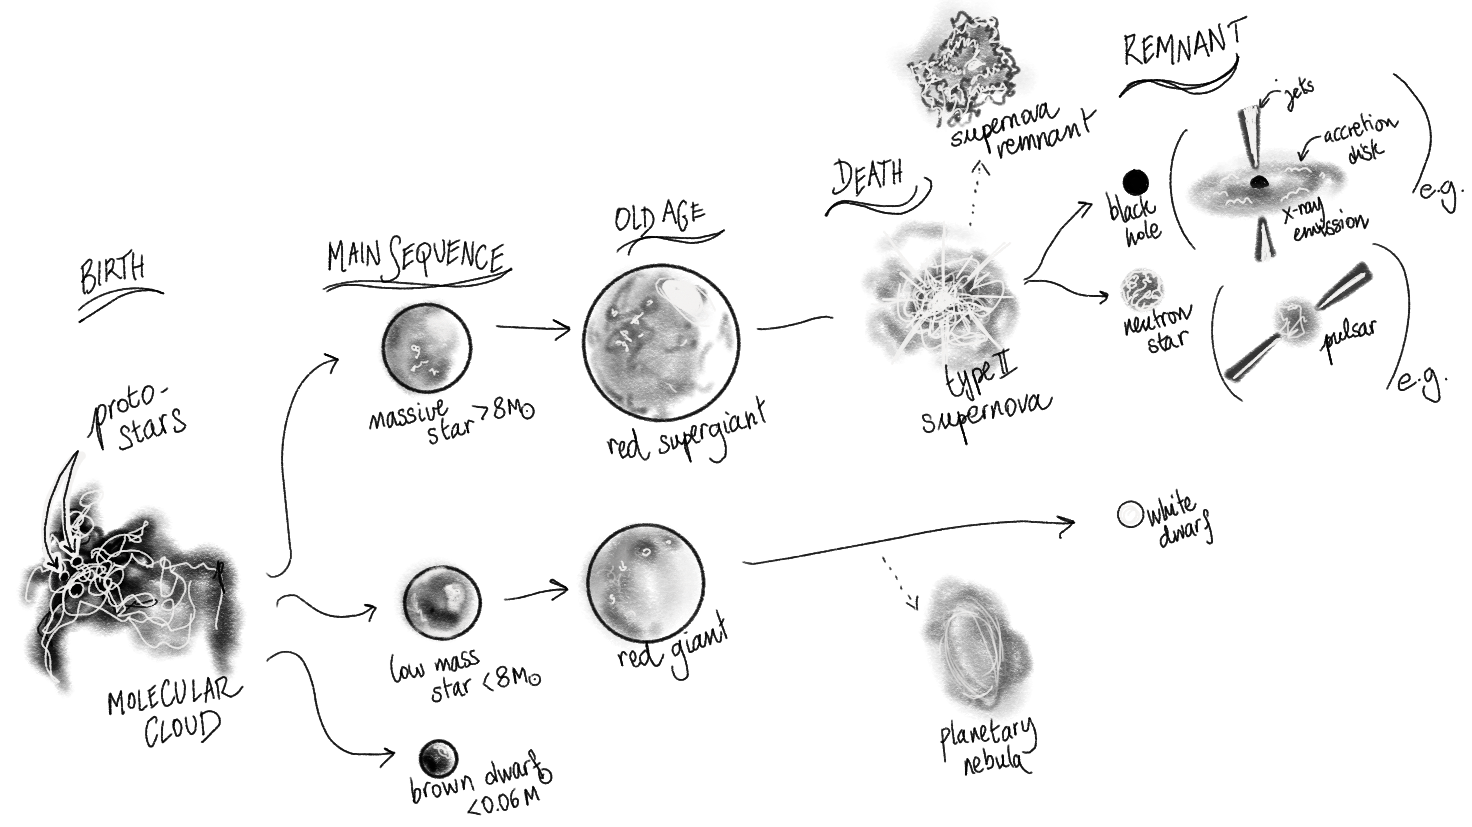
\includegraphics[width=\linewidth]{img/stellar_cycle.png}
    \caption{The different stages of stellar evolution as a function of the main sequence star's mass.}
    \label{fig:stellar_cycle}
\end{figure}


\subsection{Astrophysical Transients}

Astrophysical transients are cosmic events characterized by their changing brightness over relatively short time periods. These phenomena stem from a variety of astrophysical sources and each type of transient showcases distinct characteristics. In this section, we will delve into several types of transients. It's important to note, however, that the array of transients we discuss here represents only a portion of the myriad transient phenomena observable in our universe.

\subsubsection{Supernovae (SNe)}

Supernovae (SNe) rank as some of the universe's most powerful and luminous events, signaling the explosive and dramatic demise of stars. These cosmic explosions can occur in one of two primary ways. The first involves massive stars at the end of their life cycle. When such a star exhausts its nuclear fuel, its core collapses under the force of gravity, triggering a violent explosion. This type of supernova is known as a core-collapse supernova.

The second type, known as a Type Ia supernova, occurs in binary star systems where a white dwarf star accretes matter from its companion. Once the white dwarf reaches a critical mass, a runaway nuclear reaction ensues, leading to a spectacular explosion.

Supernovae are essential to the cosmic cycle of matter. In these stellar explosions, elements heavier than iron are synthesized and then scattered across the universe, contributing to the formation of new stars, planets, and even the building blocks of life. In terms of brightness, a supernova can briefly outshine an entire galaxy, emitting as much energy in a few months as our Sun will in its entire lifetime.

The remnants of supernovae are equally fascinating. They can leave behind dense \textbf{neutron stars} or, in the case of the most massive stars, \textbf{black holes}. The expanding shock waves from supernovae also help to shape the interstellar medium, triggering the formation of new stars.

Observations of supernovae have been pivotal in astrophysics, providing insights into stellar evolution, the interstellar medium, and cosmology. Notably, the study of distant Type Ia supernovae has been instrumental in understanding the expansion of the universe and the mysterious dark energy driving this expansion.

\subsubsection{Gamma-Ray Bursts (GRBs)}

Gamma-Ray Bursts (GRBs) stand as some of the most intense and energetic phenomena in the cosmos, observable in distant galaxies. They manifest as sudden, extremely bright flashes of gamma rays, the most energetic form of light. The luminosity of these bursts is so immense that, for their brief duration, they can become the brightest electromagnetic events in the visible universe.

GRBs are typically divided into two categories based on their duration: short-duration GRBs and long-duration GRBs. Short-duration bursts, lasting less than two seconds, are thought to originate from the merger of binary systems containing neutron stars. This collision results in a violent burst of energy and, often, the formation of a black hole.

On the other hand, long-duration GRBs, which last more than two seconds and can continue for several minutes, are generally associated with the deaths of massive stars. In these cases, the core of the star collapses, leading to a supernova or a hypernova, and subsequently, the formation of a black hole. The intense gamma rays are believed to be released as highly concentrated jets of energy and matter, moving at nearly the speed of light.

Despite their transient nature, GRBs leave behind afterglows in other wavelengths like X-ray, optical, and radio, offering astronomers valuable clues about their origins and the characteristics of the intervening space.

\subsubsection{Active Galactic Nuclei (AGN)}

Active Galactic Nuclei (AGN) are located at the centers of some galaxies. These compact regions significantly outshine the rest of their host galaxies, with their extraordinary luminosity originating from supermassive black holes at their cores.

The immense gravitational pull of these black holes draws in surrounding gas and dust, forming an accretion disk. As matter spirals into the black hole, it heats up to extremely high temperatures, emitting vast amounts of energy across the electromagnetic spectrum, from radio waves to visible light to X-rays. This process not only illuminates the AGN but also can impact the host galaxy's evolution.

AGNs exhibit a wide variety in their characteristics and are classified into different types based on their properties. For instance,\textbf{ quasars} are the most luminous and distant AGNs, visible across the universe, while \textbf{Seyfert galaxies} are closer and slightly less luminous. \textbf{Blazars} are another type of AGN known for their rapid and highly variable emissions, believed to be due to their jets being aligned with our line of sight.

One of the defining features of AGNs is their variability. They can change in brightness over a range of timescales, from days to years. This variability is a crucial tool for astronomers to understand the size and structure of the regions close to the black hole, as well as the dynamics of the accretion process.

\subsubsection{Tidal Disruption Events (TDEs)} 

Tidal Disruption Events (TDEs) are spectacular and violent occurrences in the cosmos, happening when a star strays too close to a supermassive black hole, typically situated at the center of a galaxy. The intense gravitational forces of the black hole exert different strengths of tidal forces on different parts of the star, ultimately pulling the star apart in a process often referred to as ``spaghettification,'' due to the elongation effect on the star's material.

As the star disintegrates, its remains — a stream of gas and stellar debris — spiral inward towards the black hole, forming a hot, rotating accretion disk. The friction and intense gravitational forces within this disk heat the material to extremely high temperatures, causing it to emit bright flares of energy, particularly in the ultraviolet and X-ray regions of the electromagnetic spectrum.

TDEs offer astronomers a rare opportunity to study the properties and environments of supermassive black holes. Since these black holes are typically quiescent, the sudden influx of material from a TDE can illuminate the black hole’s surroundings, providing valuable information about the black hole's mass, spin, and the nature of accretion processes. Additionally, TDEs can shed light on the population and distribution of stars around supermassive black holes.

\subsubsection{Fast Radio Bursts (FRBs)}
Fast Radio Bursts (FRBs) are one of the most intriguing astrophysical phenomena discovered in recent years. These are sudden and intense bursts of radio waves originating from distant parts of the universe, each lasting only a few milliseconds. Despite their brief nature, FRBs are incredibly powerful, releasing as much energy in a few milliseconds as the Sun does in nearly a century. The nature of FRBs is compounded by their seemingly random occurrence in the sky and the wide range of frequencies they cover.

The exact origins of FRBs remain one of the great mysteries in astronomy. Various theories have been proposed, ranging from highly magnetized neutron stars and black hole events to more exotic possibilities like cosmic strings or even \textit{alien technology} (although most astronomers agree this is the least likely possibility)!

Some FRBs have been observed to repeat, coming from the same location multiple times, while others appear as singular events. The repeaters have provided vital clues, suggesting that at least some FRBs are likely linked to highly energetic and dynamic astrophysical objects like neutron stars in extreme environments.

\subsubsection{Kilonovae}
Kilonovae represent a relatively new and exciting class of cosmic events, characterized by their luminous outbursts. These spectacular phenomena are the result of the merger of two neutron stars or a neutron star with a black hole. Unlike typical supernovae, which are driven by the collapse of a massive star, kilonovae are powered by the immense gravitational energy released during these compact object mergers.

The collision of neutron stars or a neutron star with a black hole triggers a cascade of nuclear reactions, resulting in the synthesis of heavy elements like gold, platinum, and uranium. This process, known as rapid neutron capture or the r-process, is thought to be a primary source of many heavy elements in the universe. The material ejected in a kilonova explosion is rich in these newly formed elements, and as it expands and cools, it emits a distinct signature of light. This light is typically in the infrared part of the spectrum, different from the optical emissions seen in traditional supernovae.

Kilonovae were largely theoretical until the historic observation of a neutron star merger in 2017, detected both in gravitational waves (\textbf{GW170817}) and electromagnetic radiation. This event marked the first time a cosmic event was observed in both gravitational waves and light, opening a new era of multi-messenger astronomy.

\subsubsection{Novae}

Novae occur in binary star systems, where a white dwarf and a companion star orbit each other closely. They are significantly less energetic compared to the colossal explosions of supernovae, but they are still very notable events in the cosmos. A typical nova can increase in brightness by a factor of thousands to hundreds of thousands over a few days, making them visible to the naked eye and allowing astronomers to study them in detail.

The process leading to a nova begins when the \textbf{white dwarf} starts pulling in material, typically hydrogen, from a very close by neighboring star, called its \textbf{companion star}. This material accumulates on the white dwarf's surface, gradually increasing in pressure and temperature.

As the layer of accreted material grows thicker and hotter, it eventually reaches a critical point where its temperature is high enough to ignite nuclear fusion reactions. Unlike the prolonged fusion process in the core of a regular star, this fusion occurs explosively on the surface of the white dwarf in a burst of energy. The result is a thermonuclear explosion that causes the white dwarf to suddenly brighten dramatically, emitting a vast amount of light and energy. This explosive event is what we observe as a nova.

The aftermath of a nova explosion often leaves behind an expanding shell of gas, which is ejected at high speeds from the white dwarf's surface. Over time, this shell disperses into the interstellar medium, contributing to the enrichment of the galaxy with heavier elements.
